\chapter{Modelowanie fizyczne}
W odniesieniu do syntezy dźwięku, modelowanie fizyczne polega na opisaniu zależności fizycznych występujących w trakcie gry na danym instrumencie. Niektóre z nich skupiają się na własnościach materiałowych, inne opisują interakcję fizyczną instrumentalisty z instrumentem. Generowanie fali dźwiękowej za pomocą takiego modelu opiera się na wykorzystaniu równań matematycznych oraz odpowiednich algorytmów pozwalających na scalenie wszystkich wykorzystywanych w danym momencie metod. Istnieją różne postacie opisów modeli fizycznych instrumentów:
\begin{itemize}
	\item równania różniczkowe,
	\item synteza falowodowa,
	\item modelowanie reakcji masy,
	\item przestrzeń stanów,
	\item transmitancja.
\end{itemize}

W niniejszym rozdziale opisano działanie syntezy falowodowej, która miała bardzo duże znaczenie w rozwoju modelowania fizycznego instrumentów. Jest to zarazem jedyna z metod modelowania fizycznego, która jest implementowana w urządzeniach komercyjnych, takich producentów jak Yamaha czy Korg. W kolejnych podrozdziałach przedstawiono syntezę dźwięku skrzypiec oraz fletu na podstawie schematów falowodowych. Opisano również implementację tej metody na procesorze DSP.


\section{Synteza falowodowa}
W instrumentach muzycznych proces generowania dźwięku opiera się na pojęciu fal bieżących wewnątrz drgających obiektów. Wykorzystując ich fizyczny opis, można zasymulować ich działanie za pomocą odpowiedniego algorytmu. Na tej zasadzie działa metoda cyfrowych falowodów (ang. digital waveguide). Pozwala ona na symulowanie  rozchodzenia się fal bieżących w~elementach instrumentów takich jak struna gitary czy tuba instrumentu dętego. Metoda ta została zaproponowana przez Juliusa O. Smitha z Uniwersytetu Stanforda w latach 90. Od tego czasu służy do syntezy brzmień takich instrumentów jak gitary, instrumenty smyczkowe czy instrumenty dęte.

%\section{Linia opóźniająca}
Do opisu cyfrowego falowodu potrzebna jest znajmość pojęcia linii opóźniającej (ang. delay line). Jest to element wprowadzający opóźnienie czasowe pomiędzy próbkami, które do niego wchodzą, a próbkami, które z niego wychodzą. 
\begin{figure}[H]
	\centering
	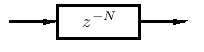
\includegraphics[width=5cm]{grafiki/linia}
	\captionsetup{justification=centering}
	\caption{Linia opóźniająca o długości N.}
	\label{rys:delay_line}
\end{figure}
Na rysunku \ref{rys:delay_line} zobrazowana została linia opóźniająca o długości $N$ próbek. Można ją przedstawić także jako $N$ bloków o jednostkowym opóźnieniu połączonych szeregowo (patrz rysunek \ref{rys:model_delay_line2}).
\begin{figure}[H]
	\centering
	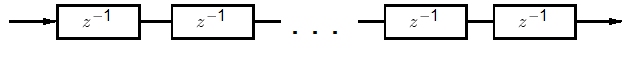
\includegraphics[width=10cm]{grafiki/model_linie}
	\captionsetup{justification=centering}
	\caption{N bloków o jednostkowym opóżnieniu.}
	\label{rys:model_delay_line2}
\end{figure}
 Implementacja linii opóźniającej sprowadza się do wykorzystania tablicy o $N$ elementach oraz zmiennych wskaźników do pierwszego i ostatniego z jej elementów. Dzięki temu, opóźnianie danych w tablicy odbywa się bez konieczności przepisywania jej całej zawartości w każdej chwili czasu. W celu uzyskania opóźnień czasowych o niecałkowitą liczbę próbek, stosuje się prostą interpolację liniową pomiędzy dwoma sąsiednimi danymi.

%\section{Cyfrowy falowód}
% https://edu.pjwstk.edu.pl/wyklady/mul/scb/main37.html

Cyfrowy falowód to w uproszczeniu dwukierunkowa linia opóźniająca. Implementuje się go zatem jako dwie linie opóźniające, w których fale rozchodzą się w przeciwnych kierunkach. Linie te są ze sobą sprzężone na końcach za pomocą inwerterów. Cyfrowy falowód można interpretować na przykład jako strunę - dłuższa struna będzie wiązała się z dłuższym falowodem. Oznacza to, że można określić prędkość odchylania się struny w dowolnym punkcie jej długości. Dokonuje się tego poprzez sumowanie, w danym punkcie struny, prędkości fali rozchodzącej się w jednym kierunku oraz predkości fali rozchodzącej się w drugim kierunku.
\begin{figure}[H]
	\centering
	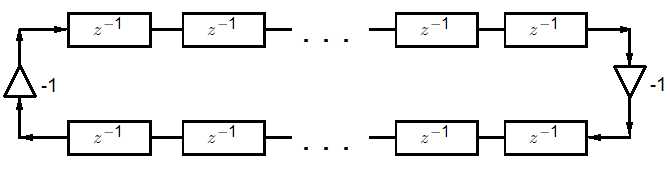
\includegraphics[width=10cm]{grafiki/model_falowod}
	\captionsetup{justification=centering}
	\caption{Cyfrowy falowód jako złożenie dwóch linii opóźniających.}
	\label{rys:model_falowod}
\end{figure}
\section{Synteza dźwięku skrzypiec}
Instrumenty smyczkowe są jedną z grup instrumentów, które modeluje się za pomocą cyfrowych falowodów. W niniejszym podrozdziale przedstawiona zostanie zasada działania syntezy dźwięku skrzypiec z wykorzystaniem właśnie tej metody, implementacja zastosowana w autorskim projekcie oraz uzyskane wyniki.

\subsection{Zasada działania syntezy dźwięku skrzypiec}
Syntezę dźwięku skrzypiec można podzielić na trzy zakresy:
\begin{itemize}
	\setlength\itemsep{-3pt}
	\item symulację interakcji pomiędzy smyczkiem a struną,
	\item symulację rozchodzenia się fal w strunie,
	\item symulację przechodzenia fal ze strun do korpusu skrzypiec poprzez mostek.
\end{itemize}
Kompletny schemat blokowy modelu realizującego syntezę dźwięku instrumentu smyczkowego został pokazany na rysunku \ref{rys:schematblokowy} pochodzącym z \cite{bowed_3}.
\begin{figure}[H]
	\centering
	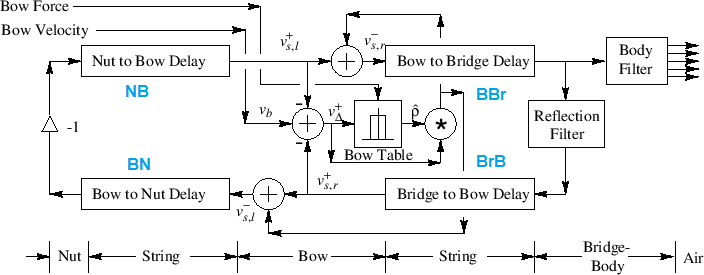
\includegraphics[width=12cm]{grafiki/schematblokowy}
	\captionsetup{justification=centering}
	\caption{Schemat blokowy modelu realizującego syntezę dźwięku \cite{bowed_3}.}
	\label{rys:schematblokowy}
\end{figure}
Poszczególne elementy skrzypiec zostały oznaczone na rysunku \ref{rys:skrzypce}.
\begin{figure}[H]
	\centering
	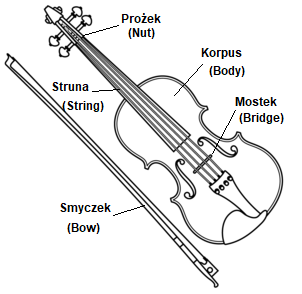
\includegraphics[width=5cm]{grafiki/skrzypce}
	\captionsetup{justification=centering}
	\caption{Elementy skrzypiec istotne dla symulacji.}
	\label{rys:skrzypce}
\end{figure}

W następnych podrozdziałach omówione zostaną kolejne obszary syntezy w oparciu o \cite{bowed_smith}. Należy mieć na uwadzę, że ostatecznie synteza tego typu przeprowadzana jest na DSP w czasie rzeczywistym.


\subsubsection{Rozchodzenie się fal w strunie}
Rozchodzenie się fal w strunie jest symulowane z wykorzystaniem cyfrowego falowodu oraz filtrów, które mają za zadanie odwzorować odbijanie się fal na jej końcach. Fale rozchodzące się w~strunie wpływają na prędkość jej lokalnych odchyleń. Ta prędkość wraz z prędkością przesuwania się smyczka po strunie stanowią podstawę do syntezy dźwięku skrzypiec. 


%\subsubsection{Odbicia na końcach struny}
Fale w strunie rozchodzą się w obu kierunkach, aż dotrą do końca struny - mostka, prożka lub palca skrzypka. Elementy te, oznaczone na rysunku \ref{rys:skrzypce}, uniemożliwiają strunie ruch, zatem fale się od nich odbijają. Fala, która dociera do jednego z tych elementów, zostaje częściowo odbita, więc zmienia się jej kierunek rozchodzenia. Odbijanie implementowane jest jako przepisywanie danej próbki z końca jednej linii opóźniającej do początku drugiej w obrębie jednego cyfrowego falowodu. Przy takim odbiciu następuje zmiana znaku próbki.
Dodatkowo, aby uwzględnić straty zależne od częstotliwości zachodzące przy odbiciach oraz samym rozchodzeniu się fali, co najmniej jedno odbicie modeluje się za pomocą filtra dolnoprzepustowego o wzmocnieniu mniejszym od 1. 
Ponadto do modelowania zjawiska dyspersji można użyć filtra wszechprzepustowego \cite{allpass}.


\subsubsection{Interakcja pomiędzy smyczkiem a struną}
Smyczek przesuwany po strunie, na skutek tarcia pomiędzy jego włosiem a struną, wprawia ją w ruch. Dopóki siła tarcia jest większa niż siła sprężystości struny, to struna odchyla się zgodnie z~ruchem smyczka. Jednak w momencie kiedy siła sprężystości będzie odpowiednio duża, struna przestanie podążać za smyczkiem i wykona gwałtowny ruch w kierunku przeciwnym do przesuwania smyczka.  Cykl ten powtarza się przez cały czas trwania pojedynczego jednokierunkowego ruchu smyczka po strunie.  \\
Do modelowania tego zjawiska wykorzystuje się współczynnik odbicia $\rho$, który powstał na podstawie opisu tarcia pomiędzy struną a smyczkiem \cite{bowed_3}. Jego wykres przedstawiono na rysunku \ref{rys:tarcie}. Przy wartości współczynnika odbicia $\rho$ równej $1$, struna podąża za smyczkiem. Im wartość $\rho$ jest mniejsza, tym większy jest poślizg struny.
\begin{figure}[H]
	\centering
	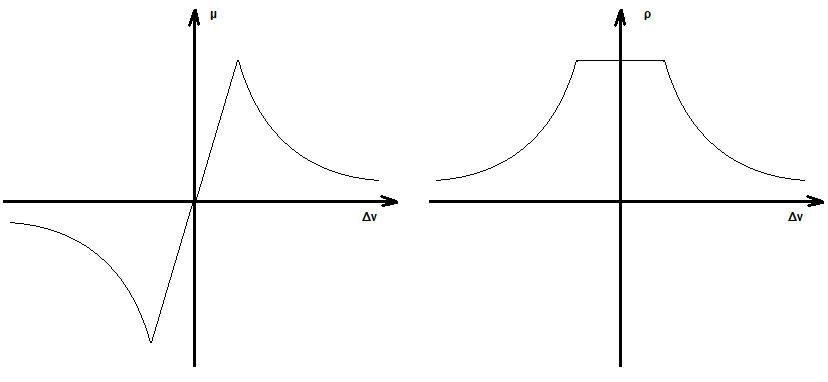
\includegraphics[width=8cm]{grafiki/tarcie2}
	\captionsetup{justification=centering}
	\caption{Współczynnik odbicia $\rho(\Delta v)$.}
	\label{rys:tarcie}
\end{figure}
Wartości współczynnika odbicia $\rho$ są wyliczane raz, według wzoru
\begin{equation} \label{equ:model_wsp_odbicia}
\rho(\Delta v) = \left \{\begin{array}{ r l }
0.98, & \quad \text{dla } (|3 (\Delta v + 0.001) | + 0.75)^{-4} > 0.98\\
0.01, & \quad  \text{dla } (|3 (\Delta v + 0.001) | + 0.75)^{-4} < 0.01\\
(|3 (\Delta v + 0.001) | + 0.75)^{-4}, & \quad \text{w pozostałych przypadkach.}
\end{array}
\right.
\end{equation}
\begin{tabular}{ l l l l}
	gdzie: & $\Delta v$ &  - & różnica prędkości pomiędzy smyczkiem a struną.
\end{tabular} \\ \\
i przechowywane w tablicy. Następnie wyznacza się różnicę pomiędzy prędkościami struny oraz smyczka $v_{diff}$:
\begin{equation} \label{equ:wzor1}
v_{diff}[t] = v_b[t] - v_{l}^{+} - v_{r}^{+}
\end{equation}
\begin{tabular}{ l l l l}
	gdzie: & $t$ &  - & obecna chwila czasu, \\
	&	$v_b$ & - &  prędkość smyczka, \\
	&	$v_{l}^{+}$ & - & prędkość struny przychodząca wraz z falą z lewej strony,\\
	&	$v_{r}^{+}$ & - &  prędkość struny przychodząca wraz z falą z prawej strony.\\
\end{tabular} \\ \\
Dalej wyznaczone zostają prędkości struny, które rozejdą się od smyczka odpowiednio w lewą i prawą stronę:
\begin{equation} \label{equ:wzor2}
v_{l}^{-} = v_r^{+} +  \rho(v_{diff}[t])v_{diff}[t]
\end{equation}
\begin{equation} \label{equ:wzor3}
v_{r}^{-} = v_l^{+} +  \rho(v_{diff}[t])v_{diff}[t]
\end{equation}
\begin{tabular}{ l l l l}
	gdzie: & $\rho(v)$ &  - & stablicowana funkcja przedstawiona na rysunku \ref{rys:tarcie}. \\
	
\end{tabular}
\vspace{6pt}

W wyniku pobudzania smyczkiem, struna wpada w charakterystyczny ruch, który jest nazywany ruchem Helmholtza. Jak pokazano w \cite{bowed_2}, próbkowanie prędkości wychyleń struny - będącej w~ruchu Helmholtza - w danym punkcie jej długości, daje sygnał zbliżony do przebiegu piłokształtnego. Zgadza się to z wcześniej opisanym zjawiskiem cyklicznego podążania struny za smyczkiem oraz ślizgania się po nim.

\subsubsection{Przechodzenie fal ze strun do korpusu skrzypiec}\label{sec:model_violinarma}

Ostatnim etapem jest przenoszenie się fal akustycznych ze strun do korpusu skrzypiec, które zachodzi w mostku. Później drgający korpus wprowadza te fale do powietrza i tak powstaje słyszalny dźwięk. W tym celu bada się funkcję przenoszenia pomiędzy mostkiem a powietrzem. 

W \cite{bowed_smith} do zbadania transmitancji mostek-korpus, zaproponowano metodę, w której sygnałem wyjściowym jest dźwięk w powietrzu, a sygnałem wejściowym jest siła działająca na mostek. Przyjęcie siły jako sygnału na wejściu tego układu wynika z tego, że mostek jest nieruchomym mocowaniem struny. Zatem prędkość mostka jest znikoma. Na mostek unieruchamiający wibrującą strunę działa siła wynikająca z prędkości odchyleń tej struny. W przytoczonej pracy, do pomiaru dźwięku został wykorzystany mikrofon, umieszczony w odległości około 30cm (jedna stopa) od czoła instrumentu, oraz przetwornik piezoelektryczny, przyklejony żywicą epoksydową do mostka, co pokazano na rysunku \ref{rys:pomiary}. Aby uzyskać jak najlepszy stosunek sygnału do szumu sygnału wyjściowego, mikrofon nie mógł znajdować się zbyt daleko oraz same pomiary powinny być przeprowadzane w komorze bezechowej.

\begin{figure}[H]
	\centering
	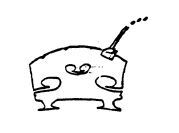
\includegraphics[width=5cm]{grafiki/pomiary}
	\captionsetup{justification=centering}
	\caption{Przetwornik piezoelektryczny przyklejony do mostka skrzypiec \cite{bowed_smith}.}
	\label{rys:pomiary}
\end{figure}

Autor \cite{bowed_smith} dokonał prób z rozmaitymi sposobami pobudzania struny: prostego smyczkowania, techniki glissando, ze strunami owiniętymi tkaniną (próbowano uchwycić szum, syczenie smyczka lekko przesuwanego po strunie w pobliżu mostka), uderzania przetwornika śrubokrętem oraz szarpania strun kostką gitarową w pobliżu mostka. Najlepsze wyniki otrzymano ostatnim sposobem.

Uzyskane w ten sposób widmo częstotliwościowe poddano odpowiedniej obróbce. Między innymi zmniejszono częstotliwość próbkowania oraz wygładzono przebieg widma. Następnie próbowano dopasować do niego proces autoregresyjny używając różnych metod identyfikacji. Najlepszy wynik uzyskano stosując normę Hankela, a końcowe dopasowanie uzyskanych charakterystyk pokazano na rysunku \ref{rys:hankel}.

\begin{figure}[H]
	\centering
	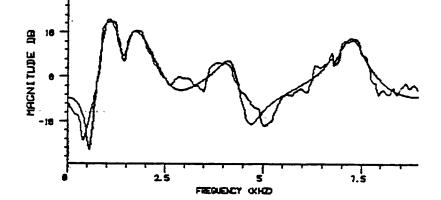
\includegraphics[width=8cm]{grafiki/hankel}
	\captionsetup{justification=centering}
	\caption{Dopasowanie widma amplitudowego procesu AR do pomierzonego \cite{bowed_smith}.}
	\label{rys:hankel}
\end{figure}

Autorzy \cite{bowed_4} przeprowadzili podobne pomiary, z tym, że strunę pobudzali młotkiem wyposażonym w piezoelektryczny miernik siły, a mikrofon umieścili metr od instrumentu.

W \cite{bowed_2} pomiarów dokonano nieco inaczej. W opisanej tam metodzie, wykorzystany został młotek wyposażony w czujnik siły. Młotkiem tym uderzano w mostek w kierunku prostopadłym do strun. Na mostku z kolei, zamontowany był akcelerometr mierzący przyspieszenie również w~kierunku prostopadłym do strun.

Wszystkie te działania zmierzały do zidentyfikowania modelu autoregresyjnego, który odwzorowuje szczyty rezonansowe pomierzonego widma częstotliwościowego. Model ten jest pobudzany sygnałem uzyskanym z próbkowania prędkości struny. Uzyskany w ten sposób sygnał wyjściowy to model dźwięku skrzypiec.

\subsection{Implementacja syntezy dźwięku skrzypiec}
Schemat z rysunku \ref{rys:schematblokowy} na potrzeby implementacji można nieco uprościć. Przekształcając schemat, dwie linie opóźniające (BN i NB) rozdzielone jedynie inwerterem można połączyć w~jedną (DL1), której znak jest zmieniany na końcu. Tak samo można zrobić z dwoma liniami opóźniającymi rozdzielonymi filtrem dolnoprzepustowym (BBr i BrB). Takie działania nie mają wpływu na efekt końcowy syntezy, a dzięki nim zaimplementować trzeba tylko dwie linie opóźniające, zamiast czterech. Ponadto można zrezygnować z elementu modelu związanego z wpływem siły nacisku smyczka na strunę. Uproszczony schemat blokowy został pokazany na rysunku \ref{rys:model_violin_schemat}.
\begin{figure}[H]
	\centering
	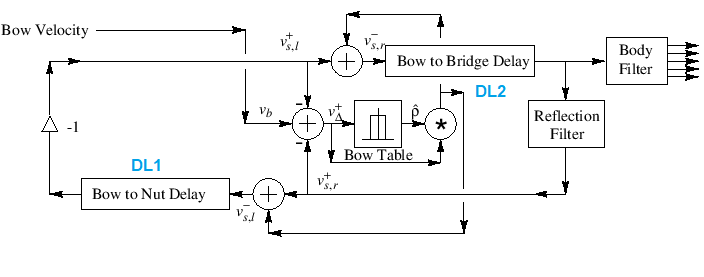
\includegraphics[width=12cm]{grafiki/model_violin_schemat}
	\captionsetup{justification=centering}
	\caption{Uproszczony schemat blokowy syntezy falowodowej skrzypiec.}
	\label{rys:model_violin_schemat}
\end{figure}
Dzięki takiej redukcji bloków funkcjonalnych, zaimplementować należy tylko dwie linie opóźniające: bridgeDelay[.] i neckDelay[.]. Długość pojedynczej linii (liczba elementów tablicy) zależy od częstotliwości najniższego z generowanych tonów i jest całkowitą częścią wielkości opisanej wzorem:
\begin{equation} \label{equ:model_ndelays}
L_{DL} = \frac{F_s}{F_{lowest}}
\end{equation}
\begin{tabular}{ l l l l}
	gdzie: & $F_{lowest}$ &  - & najniższa generowana częstotliwość. \\
\end{tabular}\\
Z linią opóźniającą skojarzone są zmienne przechowujące indeksy początkowe i końcowe linii: całkowite inPoint i outPoint oraz zmiennoprzecinkowy outPointer. 
\begin{figure}[H]
	\centering
	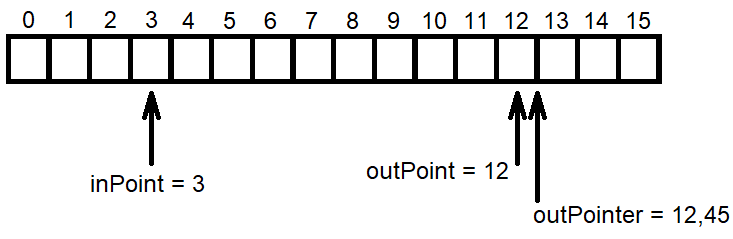
\includegraphics[width=10cm]{grafiki/model_violin_wskazniki}
	\captionsetup{justification=centering}
	\caption{Schemat linii opóźniającej i jej wskaźników.}
	\label{rys:model_violin_wskazniki}
\end{figure}
Na rysunku \ref{rys:model_violin_wskazniki} przedstawiono schemat linii opóźniającej i opisane wskaźniki. W każdej chwili czasu wskaźniki te są inkrementowane (przykład dla neckDelay[.]):
\begin{equation} \label{equ:model_wskazniki}
\text{neck\_inPoint} \gets \left \{ 
\begin{array}{ l l}
\text{neck\_inPoint+1} &  \text{gdy neck\_inPoint}+1 < L_{DL} \\
0 &  \text{gdy neck\_inPoint}+1 \geqslant L_{DL}
\end{array},
\right.
\end{equation}
\begin{equation} \label{equ:model_wskazniki2}
\text{neck\_outPoint} \gets \left \{ 
\begin{array}{ l l}
\text{neck\_outPoint+1} &  \text{gdy neck\_outPoint}+1 < L_{DL} \\
0 &  \text{gdy neck\_outPoint}+1 \geqslant L_{DL}
\end{array}.
\right.
\end{equation}
 Do komórki o indeksie inPoint wpisywana jest nowa próbka, a w komórce o indeksie outPoint zapisana jest próbka "wyjściowa". Prawdziwe wyjście linii opóźniających najczęściej nie ma całkowitego indeksu, zatem obliczane jest jako średnia ważona pomiędzy dwoma sąsiednimi próbkami. W tym celu obliczyć należy współczynnik wagowy
 \begin{equation} \label{equ:model_alpha}
\alpha_{neck} = \text{neck\_outPointer} - \text{neck\_outPoint},
 \end{equation}
który służy do wyznaczania wyjścia jako
 \begin{equation} \label{equ:model_neckoutput}
\text{neck\_output} = (1 - \alpha_{neck}) \text{neckDelay[neck\_outPoint]} + \alpha_{neck} \text{neckDelay[neck\_nextOut]}
\end{equation}
\begin{tabular}{ l l l l}
	gdzie: & neck\_nextOut & - & przyjmuje wartość: neck\_outPoint+1 lub 0. \\
\end{tabular} \\
Na końcu jednej z linii (bridgeDelay[.]) znajduje się prosty filtr dolnoprzepustowy (stringFilter). Każda wychodząca próbka poddawana jest filtracji według wzoru:
 \begin{equation} \label{equ:model_stringfilter}
\text{stringFilter[n]} = \text{SF}\_\text{g}*\text{SF}\_\text{b}*\text{bridge\_output} - \text{SF}\_\text{a}* \text{stringFilter[n-1]}.
\end{equation}
\begin{tabular}{ l l l l}
	gdzie: & \text{SF}\_\text{g} & - & wzmocnienie filtra równe 0.95, \\
			& \text{SF}\_\text{a} & - & współczynnik a filtra równy $\frac{24000}{5F_s} - 0.55$, \\
			& \text{SF}\_\text{b} & - & współczynnik b filtra równy $1+\text{SF}\_\text{a}$. \\
\end{tabular} \\
Następnie oblicza się sumę wyjść stringFilter i neck\_Output (wyjścia te dodatkowo zmieniają znak na przeciwny). Uzyskany rezultat dodawany jest do zmiennej opisującej prędkość smyczka pomnożonej przez ADSR:
 \begin{equation} \label{equ:model_deltav}
\Delta v = \text{ADSR[n]} v_b + (\text{stringFilter[n]} + \text{neck\_output})
\end{equation}
\begin{tabular}{ l l l l}
	gdzie: & $v_b$ &  - & to maksymalna prędkość smyczka osiągana w symulacji, \\
	& ADSR[n] &  - & wartość obwiedni w danej chwili czasu. \\
\end{tabular} \\
Na podstawie wartości $\Delta v$ oblicza się nową prędkość struny:
 \begin{equation} \label{equ:model_newv}
v_{new} = \rho (\Delta v) \Delta v
\end{equation}
\begin{tabular}{ l l l l}
	gdzie: & $\rho (\Delta v)$ &  - & wyznacza się korzystając z wzoru (\ref{equ:model_wsp_odbicia}). \\
\end{tabular} \\
Nowa wartość prędkości jest wprowadzana do linii opóźniających wraz z wartościami odbić:
 \begin{equation} \label{equ:model_newv2}
\text{neckDelay[neck\_inPoint]} = v_{new} - \text{stringFilter[n]},
\end{equation}
 \begin{equation} \label{equ:model_newv3}
\text{bridgeDelay[neck\_inPoint]} = v_{new} - \text{neck\_output}.
\end{equation}

Ostatnim krokiem jest filtracja wyjściowych próbek bridge\_output za pomocą procesu ARMA opisanego w części \ref{sec:model_violinarma}.
W celu uzyskania efektu Vibrato, należy w każdej chwili czasu modyfikować zmienną neck\_outPointer w rytm sygnału sinusoidalnego o niewielkiej częstotliwości. Modyfikacja ta pociąga za sobą konieczność aktualizowania współczynnika wagowego $\alpha _{neck}$ oraz wskaźnika neck\_outPoint. 
%\chapter{Implementacja syntezy dźwięku skrzypiec}
%\section{Implementacja syntezy dźwięku skrzypiec}
%\subsection{Implementacja syntezy dźwięku skrzypiec}
%\subsubsection{Implementacja syntezy dźwięku skrzypiec}
\subsection{Wyniki eksperymentalne}
Opisana implementacja pozwala wygenerować dźwięk o charakterze instrumentu smyczkowego. Na końcowe wrażenia słuchowe, poza samą syntezą falowodową, duży wpływ mają dodatkowe efekty akustyczne takie jak: odpowiednie kształtowanie obwiedni czy odpowiednio dobrany efekt Vibrato (częstotliwość, amplituda). Wyniki symulacji przeprowadzonej w środowisku Matlab przedstawiono na rysunku \ref{rys:model_violin_matlab}.
\begin{figure}[H]
	\centering
	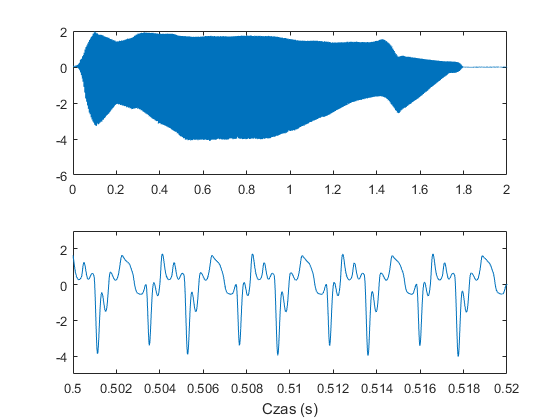
\includegraphics[width=12cm]{grafiki/model_violin_matlab}
	\captionsetup{justification=centering}
	\caption{Wygenerowany dźwięk skrzypiec. Ton o częstotliwości 240 Hz.}
	\label{rys:model_violin_matlab}
\end{figure}
